\documentclass{report}

%%% Imports %%%
% \usepackage[Lenny]{fncychap}
\usepackage{multicol}
\setlength{\columnseprule}{1pt}
\setlength{\columnsep}{1cm}
\usepackage[utf8]{inputenc}
\usepackage{XCharter}
\usepackage{float}
\usepackage[T1]{fontenc}
\usepackage{textcomp}
\usepackage[english]{babel}
\usepackage{amsmath, amssymb, amsthm}
\usepackage[a4paper, total={7.5in,10in}]{geometry}
\usepackage{blindtext}
\usepackage{hyperref}
\usepackage{graphicx}
\usepackage{empheq}
\usepackage{mdframed}
\usepackage{booktabs}
\usepackage{color}
\usepackage{psfrag}
\usepackage{bm}
\usepackage{tcolorbox}
\usepackage{bookmark}
\usepackage{tikz}
\newcommand{\warning}{
	{\fontencoding{U}\fontfamily{futs}\selectfont\char 66\relax}
}
\setlength{\parindent}{0em}
\usepackage{silence}
%Disable all warnings issued by latex starting with "You have..."
\WarningFilter{latex}{You have requested package}
%Code listing env
\usepackage{listings}
\usepackage{rust_latex/listings-rust}
\usepackage{xcolor}

\definecolor{codegreen}{rgb}{0,0.6,0}
\definecolor{codegray}{rgb}{0.5,0.5,0.5}
\definecolor{codepurple}{rgb}{0.58,0,0.82}
\definecolor{backcolour}{rgb}{0.95,0.95,0.92}

\lstdefinestyle{mystyle}{
		backgroundcolor=\color{backcolour},   
		commentstyle=\color{codegreen},
		keywordstyle=\color{magenta},
		numberstyle=\tiny\color{codegray},
		stringstyle=\color{codepurple},
		basicstyle=\ttfamily\footnotesize,
		breakatwhitespace=false,         
		breaklines=true,                 
		captionpos=b,                    
		keepspaces=true,                 
		numbers=left,                    
		numbersep=5pt,                  
		showspaces=false,                
		showstringspaces=false,
		showtabs=false,                  
		tabsize=2
}

\lstset{style=mystyle}

%%% Inkscape Integration %%%
\usepackage{import}
\usepackage{pdfpages}
\usepackage{transparent}
\usepackage{xcolor}

\newcommand{\incfig}[2][1]{%
		\def\svgwidth{#1\columnwidth}
		\import{./figures/}{#2.pdf_tex}
}

\pdfsuppresswarningpagegroup=1

%%% Define colors %%%%
\definecolor{Green}{rgb}{0.2,0.9,0.2}

%%% Title and author %%%
\author{Damian Hubert}
\title{Rust}
%%% Main Document Space %%%
\begin{document}

\maketitle
\tableofcontents


\chapter{Fondamentals}

\begin{multicols*}{2}


\section{Cargo}
\begin{itemize}
	\item Package manager, Build system, Test runner, Docs generator
\end{itemize}

\begin{tcolorbox}[title=Creating Project,colback=backcolour,size=small,left=4mm]
\begin{lstlisting}[language=bash]
cargo new "app name"
\end{lstlisting}
\end{tcolorbox}

\begin{itemize}
	\item \textbf{Cargo.toml} is the config file for the project
		\begin{itemize}
			\item \textbf{name} is independent of the directory name 
			\item \textbf{version} uses semantic versioning, see \href{https://semver.org}{this link} 
			\item \textbf{authors} should be completed by itself using git credentials 
		\end{itemize}
	\item \textbf{src} subdirecory with \textbf{main.rs} 
\end{itemize}

\begin{tcolorbox}[title=Running a Program,colback=backcolour,size=small,left=4mm]
\begin{lstlisting}[language=bash]
cargo run
\end{lstlisting}
\end{tcolorbox}

Target directory
\begin{itemize}
	\item Where cargo outputs all its build artefacts 
	\item \textbf{To add in .gitignore} 
\end{itemize}

By default, cargo compiles the project with debug symbols by default
\begin{tcolorbox}[title=Disable Debug Symbols,colback=backcolour,size=small,left=4mm]
\begin{lstlisting}[language=bash]
cargo run --release
# will be a lot faster
\end{lstlisting}
\end{tcolorbox}


\section{Variables}

\subsection{Default}

\begin{tcolorbox}[title=Structure,colback=backcolour,size=small,left=4mm]
\begin{lstlisting}[language=rust]
fn main() {
	let whatever = 2;
	// auto
	let whatever: i32 = 2;
	// specific type
}
\end{lstlisting}
\end{tcolorbox}

\begin{itemize}
	\item \textbf{let} declares a variable 
	\item Rust is a stongly typed language
		\begin{itemize}
			\item By default it will be \textbf{auto} 
			\item But a \textbf{specific} type can be specified
		\end{itemize}
\end{itemize}

\begin{itemize}
	\item \textbf{let} statements can also initialize multiple variables at once, it can de-structure the data
\end{itemize}

\begin{tcolorbox}[title=Deconstruction Example,colback=backcolour,size=small,left=4mm]
\begin{lstlisting}[language=rust]
fn main() {
	let (hello, world) = (8, 50);
}
\end{lstlisting}
\end{tcolorbox}

\subsection{Immutability}

\begin{itemize}
	\item By default, variables are \textbf{immutable} 
		\begin{itemize}
			\item \textbf{To make it mutable} add \textbf{mut} after let
		\end{itemize}
\end{itemize}

\subsection{Constants}

\begin{itemize}
	\item \textbf{const} instead of let
		\begin{itemize}
			\item The \textbf{convention} is to use\\ 
        SCREAMING\_NAMES 
			\item The type annotation is \textbf{required} here !
		\end{itemize}
	\item \textbf{Two reasons} to use const
		\begin{enumerate}
			\item A const is \textbf{global}  
			\item They're really \textbf{fast} at compile time
		\end{enumerate}
\end{itemize}


\section{Scope}

\begin{itemize}
	\item The scope is the place in the code where we are allowed to use the variables 
	\item The scope of variable is contained inside its block, and sub-blocks. If a block ends : the variable is \textbf{immediatly} dropped. 
	\item Variables can be \textbf{shadowed}, they're always \textbf{local to their scope}  
\end{itemize}

\begin{tcolorbox}[title=Shadowing,colback=backcolour,size=small,left=4mm]
\begin{lstlisting}[language=rust]
fn main() {
	let x = 5;
	{
		let x = 99;
		println!("{}", x); // prints 99
	}
	println!("{}", x); // print 5
}
\end{lstlisting}
\end{tcolorbox}

\begin{tcolorbox}[title=Shadowing in the same scope,colback=backcolour,size=small,left=4mm]
\begin{lstlisting}[language=rust]
let mut x = 5;
let x = x; // is now immutable
// can also be done to modify the type of the variable
\end{lstlisting}
\end{tcolorbox}


\section{Memory Safety}
\begin{itemize}
	\item Variables must be initialized to a value before compiling 
	\item The compiler must be sure that the variable will have a value assigned to it
\end{itemize}


\section{Functions}

\begin{itemize}
	\item Naming convention : \textbf{sneak\_cases}
\end{itemize}

\begin{tcolorbox}[title=Functions doesn't have to appear before we call them,colback=backcolour,size=small,left=4mm]
\begin{lstlisting}[language=rust]
fn main() {
	do_stuff();
}
fn do_stuff() {
}
// is valid !
\end{lstlisting}
\end{tcolorbox}

\begin{itemize}
	\item Functions \textbf{parameters} are defined with \textbf{(name: type, other variables)} 
	\item Specify the return type by adding \textbf{-> type}  
\end{itemize}

\begin{tcolorbox}[colback=backcolour,size=small,left=4mm]
\begin{lstlisting}[language=rust]
fn do_stuff(qty: f64, oz: f64) -> f64 {
	return qty * oz;
	// The short hand for returning values is to leave the ";" off
	qty * oz
}
\end{lstlisting}
\end{tcolorbox}

\begin{itemize}
	\item Leaving the ";" off the last expression in a block, will make it be returned as the value of the block
	\item There isn't support for named arguments, so all the values must be provided in the \textbf{correct order}
	\item A single function doesn't support variable numbers of arguments or $\not =$ for the same arguments
		\begin{itemize} 
			\item But macro such as \textbf{println!} do ! 
			\item The name of a macro always end with a "!"
		\end{itemize}
\end{itemize}

\section{Module System}

We create a library called \textit{lib.rs} 

\begin{tcolorbox}[title=,colback=backcolour,size=small,left=4mm]
\begin{lstlisting}[language=rust]
hello
--Cargo.toml
--src
  -- lib.rs // the hello library
  -- main.rs // the hello binary
\end{lstlisting}
\end{tcolorbox}

\begin{tcolorbox}[title=In lib.rs,colback=backcolour,size=small,left=4mm]
\begin{lstlisting}[language=rust]
fn greet() {
  println!("Hi");
}
\end{lstlisting}
\end{tcolorbox}

\begin{tcolorbox}[title=To call it in main.rs,colback=backcolour,size=small,left=4mm]
\begin{lstlisting}[language=rust]
fn main() {
  hello::greet(); //absolute path, wont work yet
  }
// because all items in a library are private by default
--> pub fn...
\end{lstlisting}
\end{tcolorbox}

\begin{itemize}
  \item Absolute path is library name (same as project), here : \textit{hello}, + scope operator :: and then name of the function 
  \item We need to add pub in front of the function 
  \item Absolute path are \textbf{very long} so \textit{use} comes in handy
\end{itemize}

\begin{tcolorbox}[title=use,colback=backcolour,size=small,left=4mm]
\begin{lstlisting}[language=rust]
// in main
use hello::greet;
// this brings greet into scope for all of main
// hello::greet becomes greet

//we can call the Standard Library with
use std::collection::HashMap; // example
// Always available
\end{lstlisting}
\end{tcolorbox}

When things are not in the std, we search on crates.io, crate $\equiv$ package, once the name
and the name and version of the package, we can import it in Cargo.toml

\begin{tcolorbox}[title=Cargo.toml,colback=backcolour,size=small,left=4mm]
\begin{lstlisting}[language=rust]
[dependencies]
pack_name = "0.2.6"
\end{lstlisting}
\end{tcolorbox}

\end{multicols*}

\chapter{Primitive Types and Control Flow}

\begin{multicols*}{2}

\section{Scalar Types}

\begin{itemize}
  \item Integers
    \begin{itemize}
      \item unsigned starts with \textbf{u} 
      \item signed starts with \textbf{i} 
      \item they are followed by the number of bits the integer as $2^{3 \rightarrow 7}$ 
      \item Except for \textbf{usize} is the size of the platform pointer type and can represent
        every memory address in the process, vectors and arrays usually use it to index 
      \item \warning all types are not supported on all hardware 
      \item Int can be specified in a lot of ways : decimal, [0x]hex, [0o]octal, [0b]binary and byte(u8 only)[b'<utf-8 char>']
      \item They can have any number of "\_" in them, for \textbf{convenience} 
    \end{itemize}
  \item Float 
    \begin{itemize}
      \item Much simpler : f32, f64 : the \textbf{default}, more precise but can be really slow on $<$ 64bit architecture 
      \item Floating point literals follow the \textbf{IEEE-754} std, we write them like \textit{3.14159} 
    \end{itemize}
  \item Booleans 
    \begin{itemize}
      \item \textbf{bool} can be \textbf{true} or \textbf{false} 
      \item \textbf{arithmetic} wont work unless casted like "true as u8"
    \end{itemize}
  \item Characters
    \begin{itemize}
      \item \textbf{char} are always \textbf{4 bytes} -> an array of chars are always UCS-4 / UTF-32 string 
      \item Fairly useless because string are UTF-8 
      \item let my\_letter = '<anything, unicode>';
    \end{itemize}
\end{itemize}

\begin{tcolorbox}[title=Suffixe variable type,colback=backcolour,size=small,left=4mm]
\begin{lstlisting}[language=rust]
let x: u16 = 5;
// we can also suffix the literal with the wanted type
let x: 5u16; // useful when passing a literal to a generic function that could accept multiple numeric types
let x: 5_u16;
\end{lstlisting}
\end{tcolorbox}

\section{Compound Types}

They gather multiple values of other types into one

\begin{itemize}
  \item $\diamond$ \textbf{Tuple} stores multiple values of \textbf{any type} 
  \item let info = (1, 3.3, 999); 
  \item \textbf{type annotation} : let info: (u8, f64, i32) = (1, 3.3, 999); 
  \item Two ways to \textbf{access members} :
    \begin{enumerate}
      \item \textbf{dot syntax} let jets = info.0; 
      \item \textbf{all at once} let (jets, fuel, ammo) = info; \textbf{max 12 arity} 
      \item \textbf{arity} is the number of elements
    \end{enumerate}
  \item $\diamond $ \textbf{Arrays} elements in contrast has to have to \textbf{same type} 
  \item let buf = [1, 2, 3]; 
  \item let buf = [0; 3]; : value; number 
  \item let buf: [u8; 3] = [1, 2, 3]; 
  \item \textbf{Indexation} buf[0], array are \textbf{limited} to a size of \textbf{32} 
  \item Arrays lives on the stack by default and are fixed size so we'll usually use \textbf{Vec} 
\end{itemize}

\section{Control Flow}

\subsection{If expression}%
\label{sub:If expression}

\begin{itemize}
  \item Does not need () around the condition $\rightarrow$ 
  \item The condition \textcolor{red}{must} evaluate to a boolean, rust does not like type coercion 
  \item An \textbf{expression} means that it returns a value, unlike \textbf{statements} 
\end{itemize}

\begin{tcolorbox}[title=If,colback=backcolour,size=small,left=4mm]
\begin{lstlisting}[language=rust]
if num == 5 {  //everything between if and { will be the condition
  msg = "five";
} else if num == 4 {
  msg = "four";
} else {
  msg = "other";
}
// or
msg = if num == 5 {  //everything between if and { will be the condition
  "five" // ; are left off to the value get's returned like tail expressions
} else if num == 4 {
  "four"
} else {
  "other"
}; // is only necessary when we use the value of an if expression
// we cannot use return, because it only applies to function bodies
// all the block return the same type

//one line
num = if a {b} else {c};
\end{lstlisting}
\end{tcolorbox}

\subsection{Loops}%
\label{sub:Loops}

\begin{itemize}
  \item If the compilers knows a loop is \textbf{unconditional} there are some cool optimizations 
  \item by itself \textcolor{blue}{continue} and \textcolor{blue}{break} will affect their inner loop
\end{itemize}

\begin{tcolorbox}[title=Unconditional Loop,colback=backcolour,size=small,left=4mm]
\begin{lstlisting}[language=rust]
'bob: loop { // 'bob is a loop annotation
  loop {
    loop {
      break 'bob; //we use the annotation to break out of a specific loop
    }
  }
}
// continue follows the same structure
\end{lstlisting}
\end{tcolorbox}

\begin{itemize}
  \item While loop are conditional except they also \textbf{terminate} the loop when the condition eval to false
\end{itemize}

\begin{tcolorbox}[title=While Loops,colback=backcolour,size=small,left=4mm]
\begin{lstlisting}[language=rust]
while dizzy() { // has to be boolean
  // do stuff
}

//is equivalent to  

loop{
  if !dizzy() { break }
  // do stuff
}

// do while are easy to do
loop{
  // do stuff
  if !dizzy() { break }
}
\end{lstlisting}
\end{tcolorbox}

\subsection{For Loops}%
\label{sub:For .. in range}

\begin{tcolorbox}[title=For Loops,colback=backcolour,size=small,left=4mm]
\begin{lstlisting}[language=rust]
for num in [7,8,9].iter() {
  // do stuff with num
}
// the iterator we use determines the items we take and their order 
// we can stack methods like map, filter and fault

// for loops can use pattern to unpack the items they receive
for (x, y) in array.iter() {
  // do stuff with x and y
}

// in range loops
for num in 0..50 { // [i..n[
for num in 0..=50 { // [i..n]
  // do stuff with num
}

\end{lstlisting}
\end{tcolorbox}

\section{Strings}

6 types in the rust std but only 2 are \textbf{important} and \textbf{overlap} each other

\begin{itemize}
  \item \textcolor{red}{\&}\textcolor{cyan}{str} : \textcolor{red}{borrowed} \textcolor{cyan}{string slice} often refers to a string
    which is confusing because the other string type is a \textcolor{blue}{String}  
  \item A litteral string is always a \&str 
  \item The biggest $\neq$ being that the date is a \&str \textbf{cannot be modified} while the \textbf{String can} 
\end{itemize}

\begin{tcolorbox}[title=Creating String,colback=backcolour,size=small,left=4mm]
\begin{lstlisting}[language=rust]
let msg = "ab<unicode>".to_string(); // to create a string from a borrowed string slice
// or by passing a bss to String::from
let msg = String::from("ab<unicode>");
\end{lstlisting}
\end{tcolorbox}
\begin{figure}[H] 
	 \centering 
	 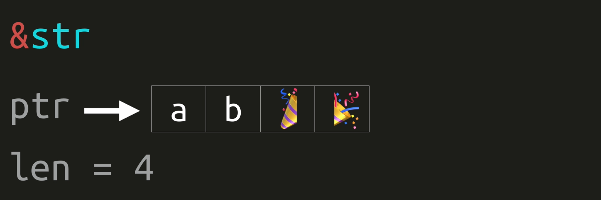
\includegraphics[width=2in]{screenshots/2022-07-15T23-25-31Z.png} 
   \caption{Are made out of a pointer to some bytes, a length, is a \textbf{subset} of a \textbf{string} }
 \end{figure}

 \begin{figure}[H] 
	 \centering 
	 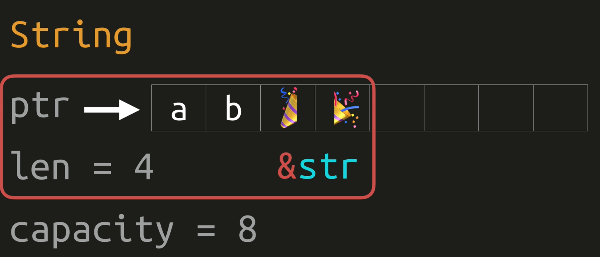
\includegraphics[width=2in]{screenshots/2022-07-15T23-28-08Z.png} 
	 \caption{Are made out of a pointer to some bytes, a length \textbf{and a capacity} that may vary upwards} 
 \end{figure}

\begin{itemize}
  \item \textbf{Both} are \textbf{valid UTF-8} by definition, compiler enforcement and runtime checks 
  \item Strings cannot be indexed by character position $\rightarrow$ lots of languages, some unicode
    takes more than a byte, a UTF-8 char can be represented by up to 4 bytes ! Diacritics are unicode that combines,
    we are searching for graphemes 
  \item Because rust emphasize on speed, indexing operations on std library collections are guaranteed to be constant time,
    this does not work with strings
\end{itemize}

\begin{tcolorbox}[title=When presented with a string,colback=backcolour,size=small,left=4mm]
\begin{lstlisting}[language=rust]
word.bytes(); //to access the vector of UTF-8 bytes, which can be indexed because bytes are fixed size
// works fine for English, without ASCII
word.chars(); //to get a iterator to iterate through Unicode scalars

unicode-segmentation !package! // providing functions that returns iterators handling graphemes 
graphemes(my_string, true)

// those solution guarantee a constant time operation
\end{lstlisting}
\end{tcolorbox}

\begin{figure}[H] 
	 \centering 
	 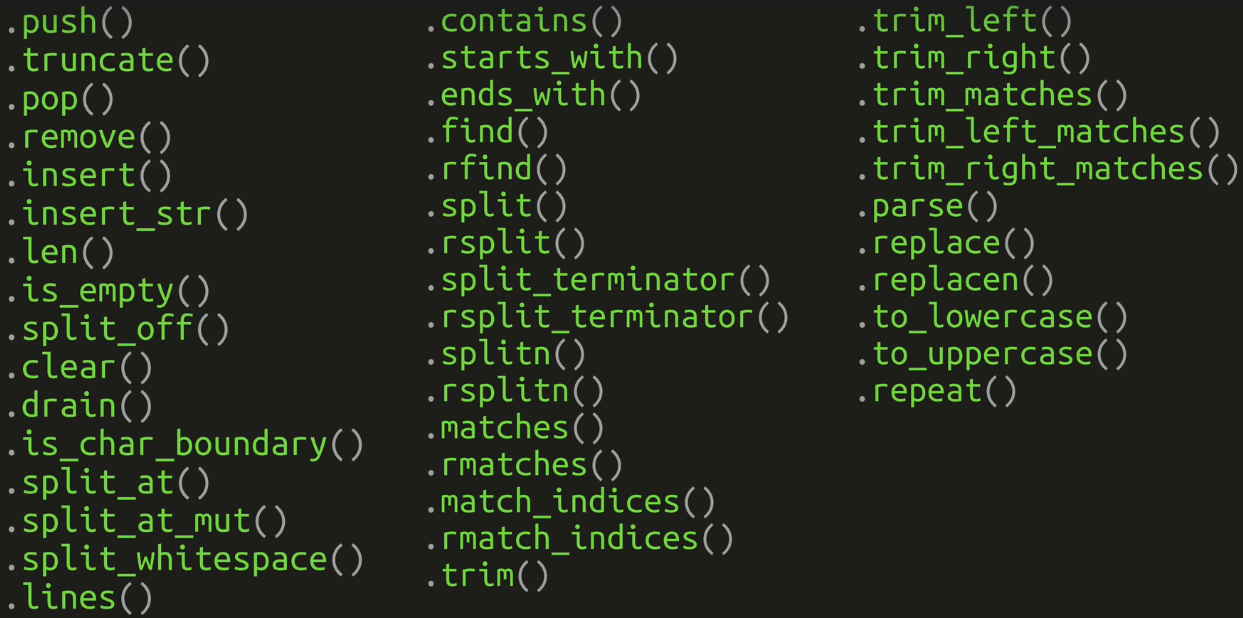
\includegraphics[width=2.8in]{screenshots/2022-07-15T23-46-36Z.png} 
	 \caption{Helper Methods} 
 \end{figure}

 \textbf{Iterators} have an handy method called \textbf{.nth(i)} that can be used to index

 \begin{itemize}
   \item \fbox{ iterator + nth = indexing }
 \end{itemize}


\begin{tcolorbox}[colback=red!5!white,colframe=red!75!black,size=small]
If an argument to pass into a function starts with a "-", cargo might try to intercept it as its own, to \textbf{prevent} that we use \textbf{double dash}, after which anything will be passed to the
program and ignored by cargo
\end{tcolorbox}


\end{multicols*}

\chapter{The Heart of Rust}

\begin{multicols*}{2}

\section{Ownership}

\begin{enumerate}
  \item \colorbox{lightgray}{Each value has an owner} : there is no
        value in memory, no data without a variable owning it 
  \item \colorbox{lightgray}{Only one owner} : No sharing of ownership
        between variables. Variables may borrow values but only one owns it
  \item \colorbox{lightgray}{Value gets dropped if its owner goes out of scope} 
\end{enumerate}

\begin{tcolorbox}[title=Ownership is action,colback=backcolour,size=small,left=4mm]
\begin{lstlisting}[language=rust]
let s1 = String::from("abc");
let s2 = s1; // s1 DOES NOT GET COPIED  because only one can own it
// s1 cannot be used anymore !
\end{lstlisting}
\end{tcolorbox}

\begin{center}
  
  \begin{tabular}{c|c}
    \textbf{Stack} & \textbf{Heap} \\
    \hline
    In order & Unordered\\
    Fixed size & Variable-size\\
    LIFO & Unordered drop\\
    Fast & Slow\\
  \end{tabular}
\end{center}

\begin{itemize}
  \item In order is possible because of fixed size 
  \item \textbf{LIFO} : last value in is the first value out 
  \item \textbf{Fast} because compact and predictable 
  \item The Heap makes it so we are always hoping arround in memory, flushing
    and reloding the cpu memory cache
\end{itemize}

  Here :
\begin{enumerate}
  \item Create s1 $\rightarrow$ [ptr $\rightarrow$ allocated bytes on the \textbf{heap} [a,b,c], len $\rightarrow$ 3, capacity $\rightarrow$ 3] appears in the stack, this makes the value of s1 
  \item We move the s1's value to s2, because we only have an owner $\rightarrow$ ptr,len,capacity gets copied from s1 and pushed as new value on the stack as part of s2. \textbf{Stopping here} would
    make memory safety \textbf{non existant}, This is why rust immediatly \textbf{invalidates} s1, while still $\exists $ on the stack, the compiler considers s1 \textbf{initialized}, wont let us use it.
    More than a shallow copy, it's a move
\end{enumerate}


\begin{figure}[H] 
	 \centering 
	 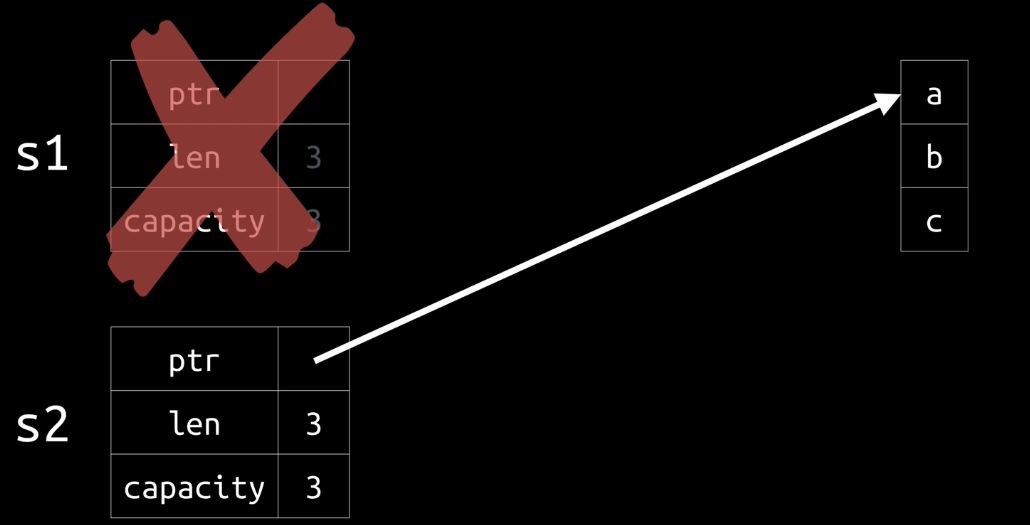
\includegraphics[width=3in]{screenshots/2022-07-16T19-12-15Z.png} 
 \end{figure}

\begin{itemize}
  \item We could still use s1 if it was \textbf{mut} and assign it a new value,
    but here, \textbf{immutable}, makes it like \textbf{garbage collector} 
\end{itemize}

\begin{tcolorbox}[title=If we don't to move but to copy the value,colback=backcolour,size=small,left=4mm]
\begin{lstlisting}[language=rust]
let s1 = String::from("abc");
let s2 = s1.clone(); //makes a copy of s1
\end{lstlisting}
\end{tcolorbox}

\begin{itemize}
  \item \textbf{Clone} instead of \textbf{copy} : Clone performs the same initial copy
    \textbf{but} then it \textbf{also} copoies the \textbf{heap date} and adjust's s2's pointer to it 
    \item Stack + Heap = Value 
    \item Copy only means stack data copy, heap data and pointer updates requires \textbf{cloning} $\equiv $ deep copy 
    \item Value dropping :
      \begin{enumerate}
        \item Run Destructor, immediatly 
        \item Free heap, immediatly 
        \item Pop stack, immediatly
      \end{enumerate}
\end{itemize}

\begin{tcolorbox}[title=Another move situation,colback=backcolour,size=small,left=4mm]
\begin{lstlisting}[language=rust]
let s1 = String::from("abc");

fn do_stuff(s: String) {
  //do stuff, returns nothing
}

do_stuff(s1); // s1 gets moved into the local variable "s" in do_stuff(), we cannot use s1 anymore

// to fix that, we could move it back
let mut s1 = String::from("abc"); 
s1 do_stuff(s1); // s gets moved back out of the function
print..s1..; error
fn do_stuff(s: String) -> String { // add return type 
  s // returns s
}
//Not a usual pattern !

// usually the function consummes the past in value
// For more often cases we should use References

\end{lstlisting}
\end{tcolorbox}

\section{References and Borrowing}

Instead of moving our variable, let's use a reference
\begin{tcolorbox}[colback=backcolour,size=small,left=4mm]
\begin{lstlisting}[language=rust]
let s1 = String::from("abc");
do_stuff(&s1); // we pass a reference to s1, do stuff no borrows a reference to the value

fn do_stuff(s: &String) { // the & indicates a reference to a type
}
\end{lstlisting}
\end{tcolorbox}

\begin{itemize}
  \item A reference allows a variable to retain the ownership of its value. Only the reference gets  moved into the function 
  \item At the \textbf{end} of func, the ref goes out of scope and gets \textbf{dropped}. The borrowing \textbf{ends} 
  \item When we create a ref to s1, rust creates a ptr to s1, rust handles their creation and destruction. References are only ptr 
  \item \textbf{Lifetimes} is a rule that \textbf{references must always be valid}, compiler wont let the creation of a reference of the date it is referencing, and no pointing to null 
  \item References defaults to \textbf{immutable} 
\end{itemize}


\begin{tcolorbox}[title=Mut ref to a mut value,colback=backcolour,size=small,left=4mm]
\begin{lstlisting}[language=rust]
let mut s1 = String::from("abc");
do_stuff(&s1); // *1
do_stuff(&mut s1); // *2

fn do_stuff(s: &String) {
  s.insert_str(0, "Hi, "); // ERROR with *1 , not with *2
  }
// now we can use ref to CHANGE the value as well
\end{lstlisting}
\end{tcolorbox}

\begin{itemize}
  \item We did not have to dereference the mutable reference in order to alter it in the do\_stuff ? 
  \item We use the same .method to access String method on a ref than we do on the value itself
    $\rightarrow$ the dot operator \textbf{auto-dereferences} down to the actual value 
  \item \textbf{Manually deref} is done by (*ref) it is required by most other operators like the \textbf{assigment} $\rightarrow$ read from or write from the actual value 
  \item This does apply to types, i32 $\rightarrow$ \&i32 and \&mut i32 
  \item x: \&mut i32 If our variable is a \textbf{mut ref} to a value, then deref x would give \textbf{mut} access to a value and the opposite.. 
  \item Since ref are implemented via \textbf{ptr}, rust has a rule to stay safe :
    We can always have \textbf{one mut ref} and \textbf{any \# of immutable refs}, applying across \textbf{all threads}  
\end{itemize}

\begin{figure}[H] 
	 \centering 
	 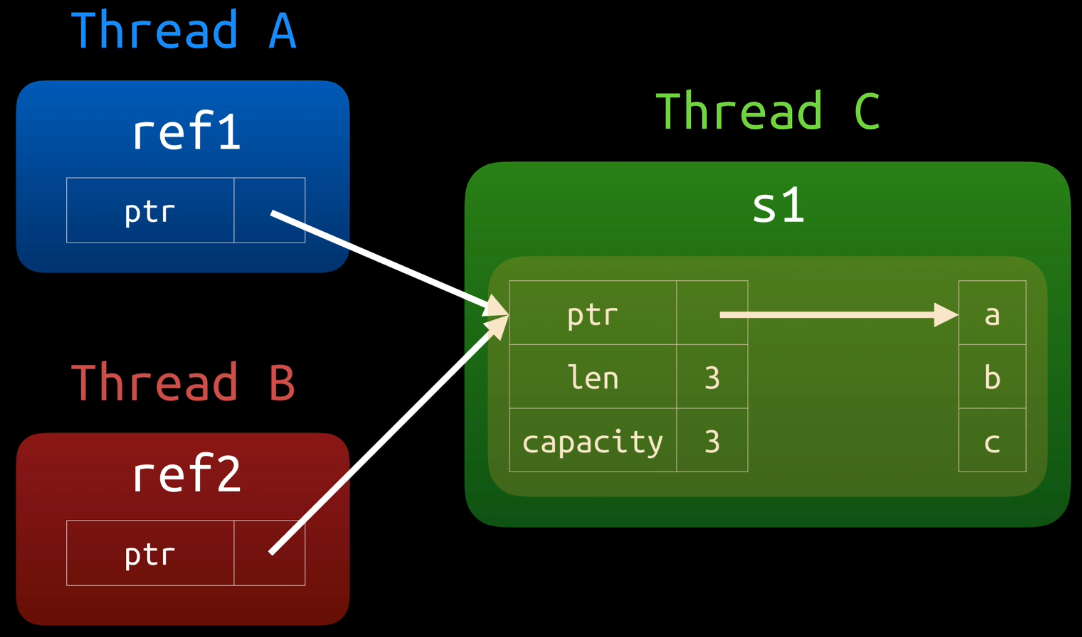
\includegraphics[width=2in]{screenshots/2022-07-16T21-38-55Z.png} 
 \end{figure}

\begin{itemize}
  \item All this rules are enforced by the compiler 
\end{itemize}


\end{multicols*}


\chapter{The Meat Of Rust}

\begin{multicols*}{2}

\begin{itemize}
  \item Structs $\equiv $ Classes 
  \item Can have [data fiels, methods, associated funcs] 
  \item Naming like \textit{AnExample} : capital-camel case 
\end{itemize}

\begin{tcolorbox}[title=Syntax,colback=backcolour,size=small,left=4mm]
\begin{lstlisting}[language=rust]
struct RedFox {
  enemy: bool,
  life: u8, // we can end the last field with "," too !
  }
\end{lstlisting}
\end{tcolorbox}

\begin{tcolorbox}[title=Init Struct,colback=backcolour,size=small,left=4mm]
\begin{lstlisting}[language=rust]
// verbose, you need to specify a value for every single field
let fox = RedFox {
  enemy: true,
  life: 70,
  }; 
// typically we implement an associated func to use as a constructor to create a struct with default values and then call that
impl RedFox {
  fn new() -> Self { // this is an associated func because it does not have a form of self as its first param
    Self { // both Self here refers to RedFox, we could also use it 
      enemy: true,
      life: 70,
    }
  }
}
\end{lstlisting}
\end{tcolorbox}

\begin{itemize}
  \item Methods and Funcs are def in an \textcolor{cyan}{impl}ementation block separate from the struct definition 
  \item \textbf{new} is a conventional name for creating a struct with \textbf{default values} 
  \item \textbf{Self} can be used in place of the struct name inside the implementation block 
\end{itemize}

\begin{tcolorbox}[title=Creating,colback=backcolour,size=small,left=4mm]
\begin{lstlisting}[language=rust]
let fox = RedFox::new(); // :: accesses a associated func in the struct
// once values are instantiated, dot syntax is used
let life_left = fox.life;
fox.enemy = false;
fox.some_method();
\end{lstlisting}
\end{tcolorbox}
\begin{itemize}
  \item "::" is the scope operator, used to \textbf{access} parts of the \textbf{namespace-like} things
\end{itemize}

\begin{tcolorbox}[title=Defining Methods,colback=backcolour,size=small,left=4mm]
\begin{lstlisting}[language=rust]
impl RedFox { // also in the impl block
  // assoc functions
  fn function()
  // methods
  fn move(self)
  fn borrow(&self)
  fn mut_borrow(&mut self)
  }
\end{lstlisting}
\end{tcolorbox}

\begin{itemize}
  \item Methods always take some form of \textbf{self} as arg 
  \item There is no stuct \textbf{inheritance}, because we have Traits
\end{itemize}

\section{Traits}

\begin{itemize}
  \item Similar to interfaces in other lang, composition $>$ inheritance 
  \item \textbf{Traits} define required behaviour, functions and methods that a struct
    must implement if it wants to have that trait
\end{itemize}

\begin{tcolorbox}[title=Example,colback=backcolour,size=small,left=4mm]
\begin{lstlisting}[language=rust]
stuct RedFox {
  enemy: bool,
  life: u32,
  }
trait Noisy {
  fn get_noise(&self) -> &str; // specifies that the struct must have a method named get_noise() returning a borrowed string slice if the struct wants to be Noisy
  }

impl Noisy for RefFox {
  fn get_noise(&self) -> &str { "Meow?" }
  } // our implementation of the get_noise method is "meow"

// Why bother doing this instead of just implementing it directly without traits ?
// Once we have trait involved, we can start writing generic functions that accept any value implementing the trait
fn print_noise<T: Noisy>(item: T) {
  println!("{}", item.get_noise());
  } // this func takes an item of type T defined to be anything that implements the Noisy trait
  // the func can use any behaviour on item that Noisy trait defines
  // This generic function can take any type as long as it satisfies the noisy trait

  // as long as one of either the trait or stuct is defined, we can implement any trait for any struct, including builtin or import types from other packages

impl Noisy for u8 {
  fn get_noise(&self) -> &str { "Byte!" }
  }

fn main() {
  print_noise(5_u8); // prints "Byte!"
  }
\end{lstlisting}
\end{tcolorbox}

\begin{itemize}
  \item Special trait called \textbf{Copy}, if our type implements copy, then it will be \textbf{copied} instead of \textbf{moved} in move situation,
    makes sense for small values fitting entirely on the stack, explaining why \textbf{simple primitive types} like int, floats and booleans implement Copy. If a type uses the \textbf{heap} then it cannot implement \textbf{Copy}. We can opt-in to impl Copy with our own types only if
    our type only uses other Copy types. 
  \item Traits implement \textbf{inheritance}
\end{itemize}

\begin{figure}[H] 
	 \centering 
	 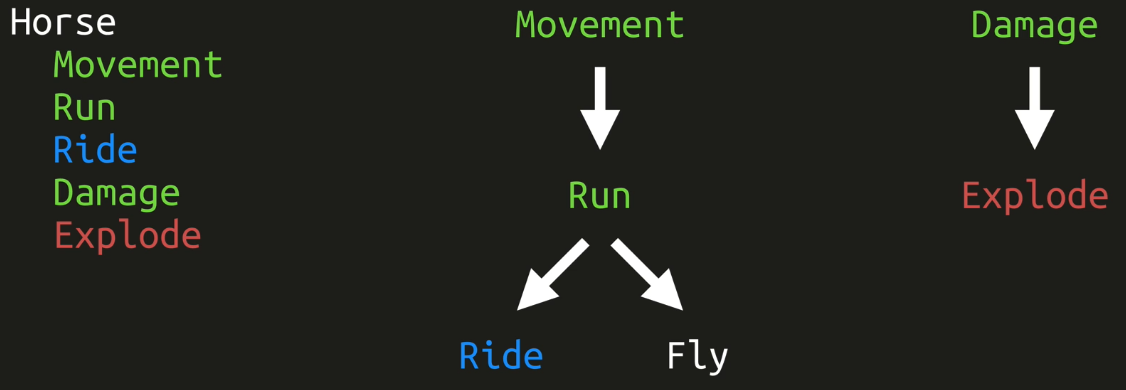
\includegraphics[width=2.5in]{screenshots/2022-07-17T11-58-25Z.png} 
 \end{figure}


\begin{tcolorbox}[title=Traits can also have default behaviours,colback=backcolour,size=small,left=4mm]
\begin{lstlisting}[language=rust]
trait Run {
  fn run(&self) {
    println!("I'm Running !")
  }
  }

struct Robot {}
impl Run for Robot {} // does not overwrite the default run method

// fully functional example

fn main() {
  let robot = Robot {};
  robot.run();
  }
\end{lstlisting}
\end{tcolorbox}

\begin{itemize}
  \item \textbf{Cannot define Fields} as part of traits, the workaround is to define setter and getter methods in our trait 
\end{itemize}

\section{Collections}

\end{multicols*}

\end{document}
